% !TeX root = ../main.tex

\chapter{Persistent Threads}\label{chapter:Persistent Threads}

Persistent GPU threads allow the hardware resources to be partitioned and reduce kernel execution and scheduling overhead.  
While the persistent \acs{GPU} threads do not allow for asynchronous programming such as with coroutines, still help ensure runtime guarantees and support execution preemption.  
Furthermore, with the entire \acs{GPU} partitioned across persistent threads, the hardware resources can be manually assigned according to the \acs{SM} number. 

To implement these persistent \acs{GPU} threads, I sought to find an open source implementation; however, I only found the LightKer implementation, used to profile persistent threads. 
The LightKer implementation implemented Mailboxes to schedule 

\begin{figure}[H]
  \centering
  \resizebox{1.0\linewidth}{!}{
	  %\documentclass[tikz, border=5mm]{standalone}
%\usepackage{tikz}
%\usetikzlibrary{shapes, arrows.meta, positioning, decorations.pathreplacing}

%\begin{document}

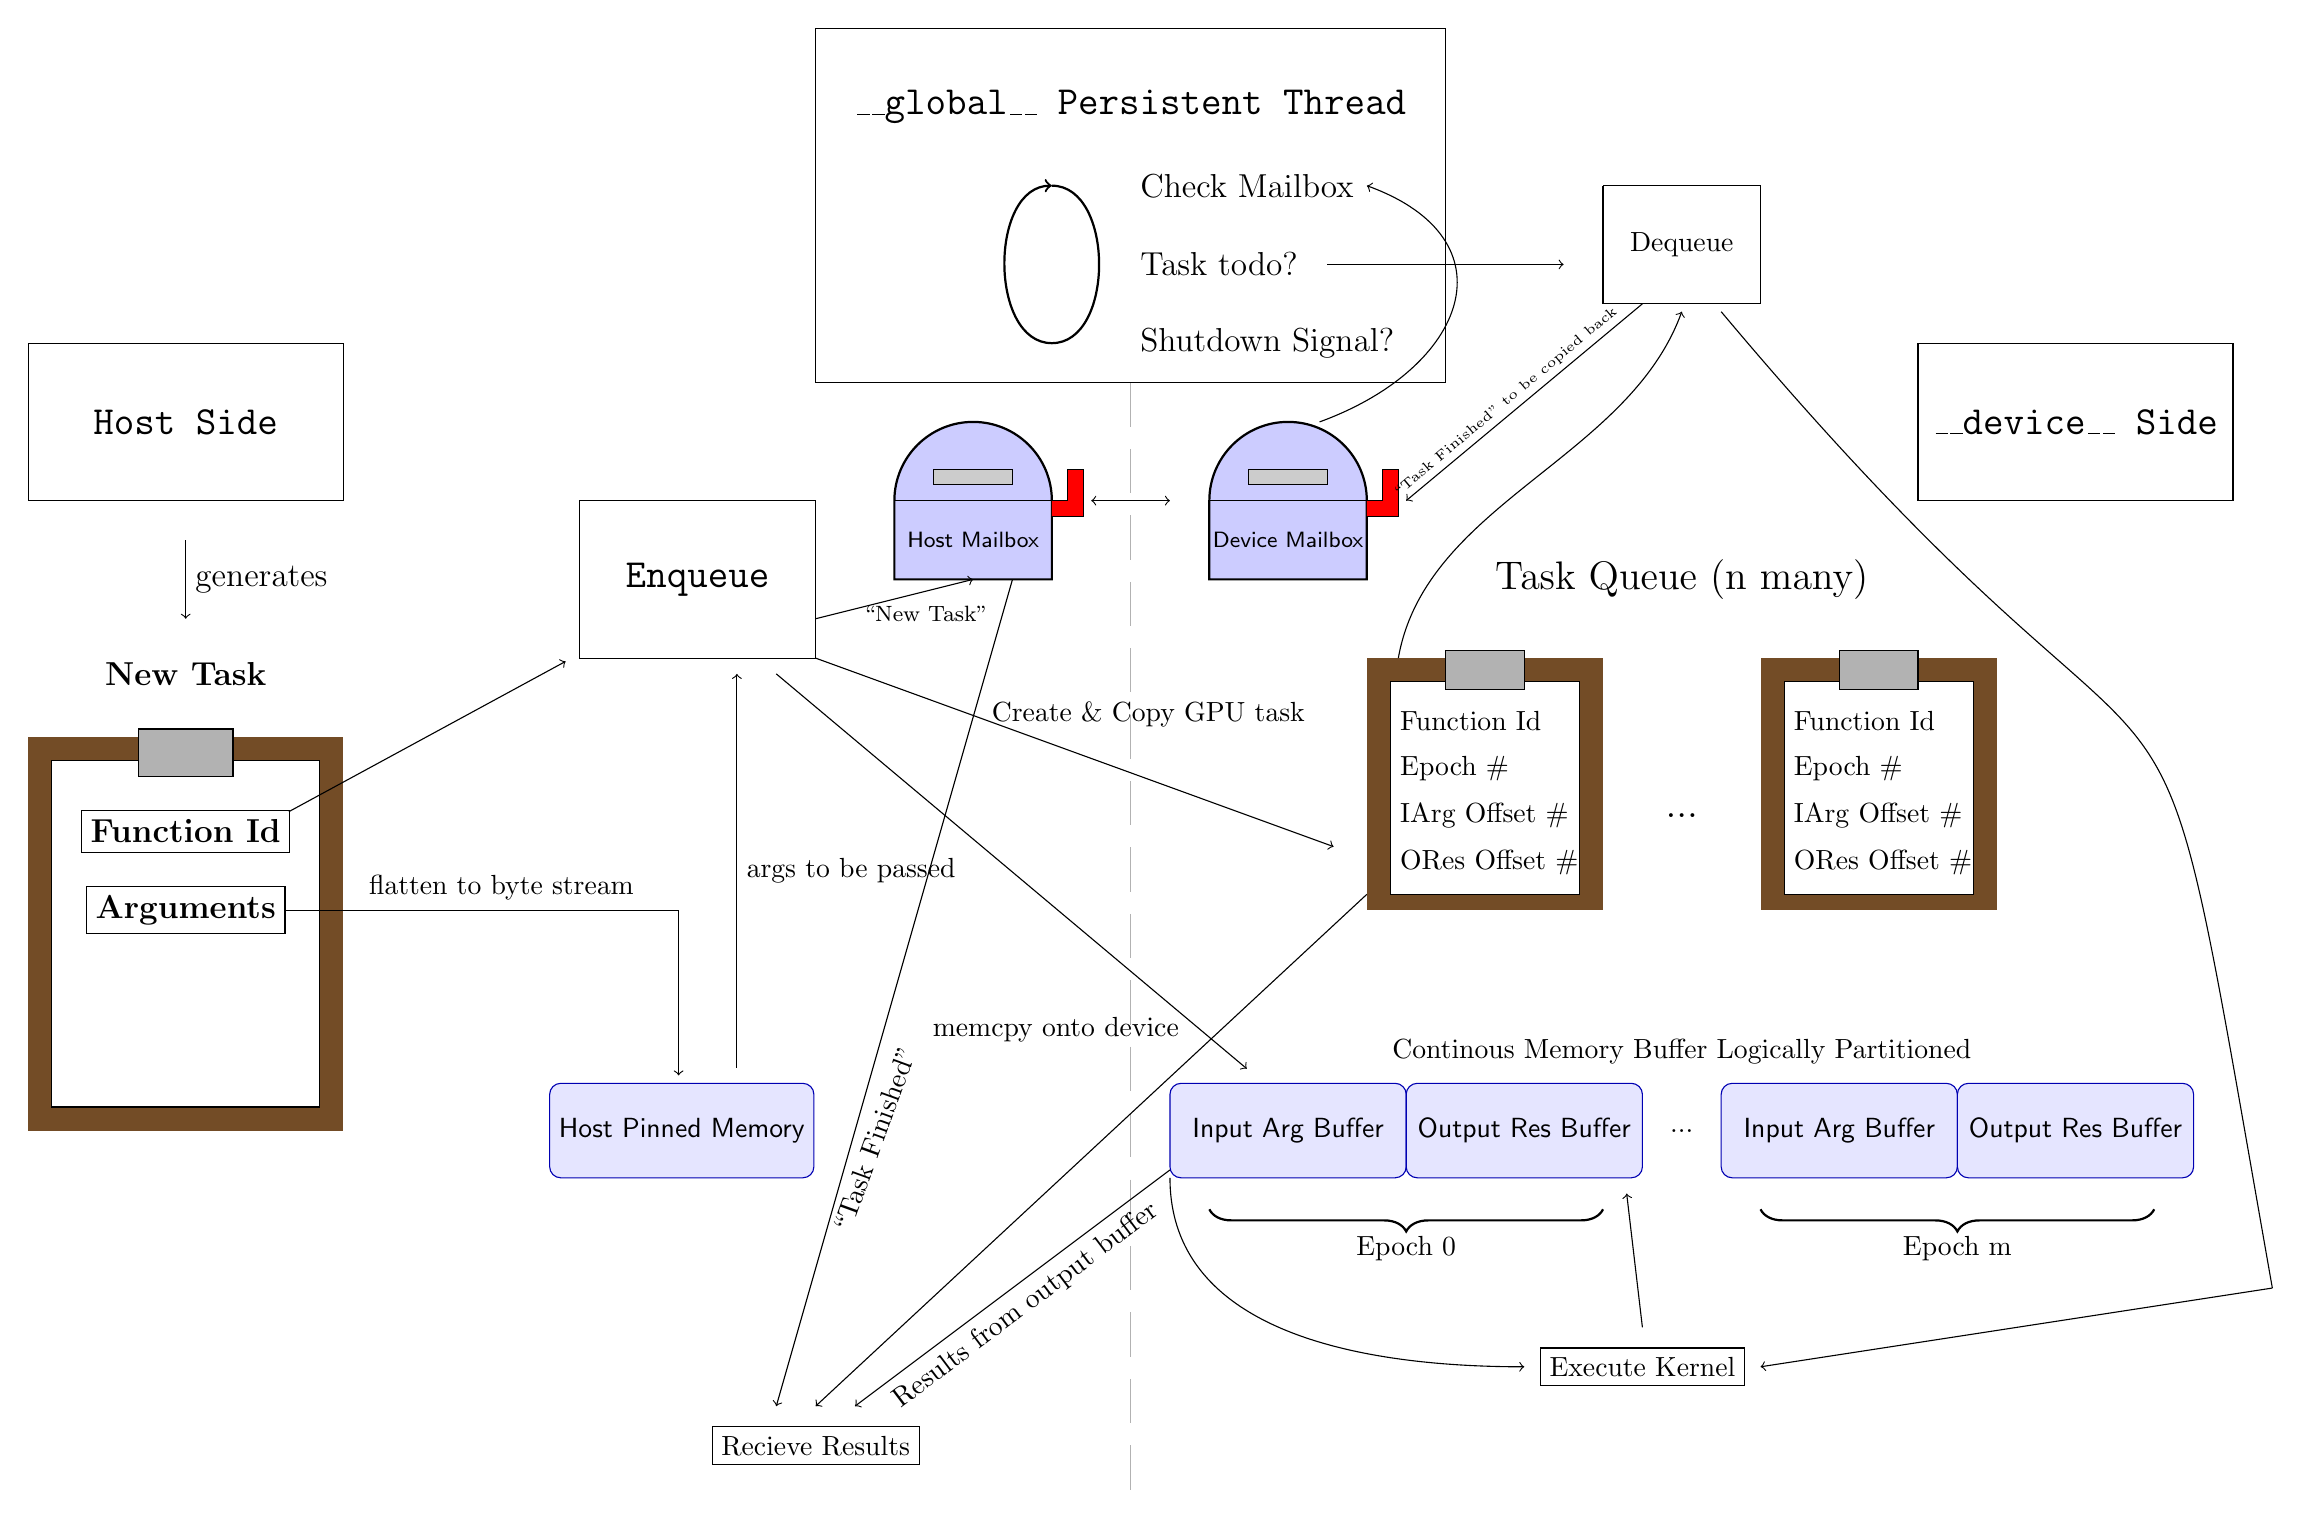
\begin{tikzpicture} [memoryblock/.style={
		draw=blue!70!black, 
		fill=blue!10, 
		rounded corners=4pt, 
		minimum width=3cm, 
		minimum height=1.2cm,
		font=\sffamily
	},
	pinicon/.style={
		symbol/.style={draw, fill=gray!40, symbol color=gray!80, symbol type=pin}
	}
	]

	%\draw[help lines] grid(32,32);


%GLOBAL BOX
	\draw[black] (12,32) -- ++(0:8) -- ++(-90:4.5) -- ++(-180:8) -- ++(-270:4.5);
	\node[minimum size=5] at (16,31) {\Large \texttt{\_\_global\_\_ Persistent Thread}};
	\node[minimum size=8, anchor=west] at (16, 29) {\large Task todo?};
	\node[anchor=west, minimum size=8] at (16, 28) {\large Shutdown Signal?};

	\node[anchor=west, minimum size=8] at (16, 30) {\large Check Mailbox};

	\draw[thick, ->]
	(15, 30)
	.. controls (15.8, 30) and (15.8, 28) .. (15, 28) 
	.. controls (14.2, 28) and (14.2, 30) .. (15, 30); 


	\draw[black, opacity=0.3,  dash pattern=on 16pt off 8pt] (16,27.5) --++(-90:14.2);

%Host Box
	\draw[black] (2, 28) --++(0:4) --++(-90:2) --++(-180:4) --++(-270:2);
	\node[ minimum size=5] at (4,27) {\Large \texttt{Host Side}};
	\draw[black ] (26, 28) --++(0:4) --++(-90:2) --++(-180:4) --++(-270:2);
	\node[ minimum size=5] at (28,27) {\Large \texttt{\_\_device\_\_ Side}};

%HOSTSIDE ARROW
	\draw[->] (4, 25.5) --++ (-90:1) node[pos=0.5, right] {\large generates};
%CLIPBOARD
	\node[font=\bfseries\large] at (4,23.8) {New Task};
	\fill[brown!60!black] (2,23) rectangle (6,18);
	\fill[white] (2.3,22.7) rectangle (5.7,18.3);
	\draw[black] (2.3,22.7) rectangle (5.7,18.3);
	\fill[gray!60] (3.4,23.1) rectangle (4.6,22.5);
	\draw[black] (3.4,23.1) rectangle (4.6,22.5);

	\node[draw, font=\bfseries\large] at (4,21.8) {Function Id};
	\node[draw, font=\bfseries\large] at (4,20.8) {Arguments};


%HOST PINNED MEM
	\node[memoryblock] at (10.3, 18) {Host Pinned Memory};
	\draw[black, ->] (5.26, 20.8) --++ (0: 5) node[pos=0.55, above] {flatten to byte stream} --++(-90: 2.1);


%ENQUEUE
	\draw[black] (9, 26) --++(0:3) --++(-90:2) --++(-180:3) --++(90:2);
	\node[minimum size=5] at (10.5,25) {\Large \texttt{Enqueue}};
	\draw[<-] (11,23.8) --++(-90:5) node[pos = 0.5, right] {args to be passed};
	\draw[->] (11.5,23.8) --++(-40:7.8) node[pos=0.9, left=4pt] {memcpy onto device};
	\draw[->] (5.31, 22.05) --++ (28.5:4);
	\draw[->] (12, 24) --++ (-20:7) node[pos=0.3,right=4pt] {Create \& Copy GPU task};


%MAILBOX HOST
	\draw[<->] (15.5, 26) -- (16.5, 26);
	\draw[thick, fill=blue!20] (13,25) -- (13,26) arc[start angle=180, end angle=0, radius=1cm] -- (15,25) -- cycle;
	\draw[fill=black!20] (13.5,26.2) rectangle (14.5,26.4);
	\draw[fill=red] (15,26) --++(0:0.2)--++(90:0.4)--++(0:0.2)--++(-90:0.6) --++(-180:0.4);
	\node at (14,25.5) {\footnotesize\textsf{Host Mailbox}};
	\draw (13,26) --(15,26);

%MAILBOX DEVICE
	\draw[thick, fill=blue!20] (17,25) -- (17,26) arc[start angle=180, end angle=0, radius=1cm] -- (19,25) -- cycle;
	\draw[fill=black!20] (17.5,26.2) rectangle (18.5,26.4);
	\draw[fill=red] (19,26) --++(0:0.2)--++(90:0.4)--++(0:0.2)--++(-90:0.6) --++(-180:0.4);
	\node at (18,25.5) {\footnotesize\textsf{Device Mailbox}};
	\draw (17,26) --(19,26);

%ARROWS to and FROM DEVICE MAILBOX
	\draw [->] (18.4, 27) to[out=20,in=-20,distance=2.0cm] (19, 30);
	\draw[->] (12, 32-7.5) -- (14,32-7) node[pos=0.7,below=2pt] {\footnotesize{``New Task''}};

%Memory Buffers
	\node at (23, 19) {Continous Memory Buffer Logically Partitioned};
	\node[memoryblock] at (18, 18) {Input Arg Buffer};
	\node[memoryblock] at (21, 18) {Output Res Buffer};

	\node[memoryblock] at (25, 18) {Input Arg Buffer};
	\node[memoryblock] at (28, 18) {Output Res Buffer};

	\node at (23, 18) {...};
	\draw[decorate, decoration={brace,mirror,amplitude=8pt}, thick] (17, 17) -- (22, 17)
	node[midway,below=6pt] {Epoch 0};

	\draw[decorate, decoration={brace,mirror,amplitude=8pt}, thick] (24, 17) -- (29, 17)
	node[midway,below=6pt] {Epoch m};

%TASK QUEUE
	\fill[brown!60!black] (19,24) rectangle (22,20.8);
	\fill[white] (19.3,23.7) rectangle (21.7,21.0);
	\draw[black] (19.3,23.7) rectangle (21.7,21.0);
	\fill[gray!60] (20,24.1) rectangle (21.0,23.6);
	\draw[black] (20,24.1) rectangle (21.0,23.6);

	\node [anchor=west] at (19.3,23.2) {Function Id};
	\node [anchor=west] at (19.3,22.6) {Epoch \#};
	\node [anchor=west] at (19.3,22.0) {IArg Offset \#};
	\node [anchor=west] at (19.3,21.4) {ORes Offset \#};

	\node at (23, 22) {\Large...};

	\fill[brown!60!black] (24,24) rectangle (27,20.8);
	\fill[white] (24.3,23.7) rectangle (26.7,21.0);
	\draw[black] (24.3,23.7) rectangle (26.7,21.0);
	\fill[gray!60] (25,24.1) rectangle (26.0,23.6);
	\draw[black] (25,24.1) rectangle (26.0,23.6);
	\node [anchor=west] at (24.3,23.2) {Function Id};
	\node [anchor=west] at (24.3,22.6) {Epoch \#};
	\node [anchor=west] at (24.3,22.0) {IArg Offset \#};
	\node [anchor=west] at (24.3,21.4) {ORes Offset \#};

	\node at (23,25) {\Large Task Queue (n many)};


%DEQUEUE
	\draw (22, 30) -- (24, 30) --++ (-90:1.5) --++(-180:2) --++ (90:1.5);
	\node at (23, 29.25) {Dequeue};
	\draw[->] (18.5, 29) --++(0:3);
	\draw [->] (19.4, 24) to[out=80,in=-110,distance=2.0cm] (23, 28.4);
	\draw [->] (22.5,28.5) -- (19.5, 26) node[pos=0, left=7pt, rotate=40] {\tiny``Task Finished'' to be copied back};


%EXECUTE Kernel
	\draw (23.5,28.4) to[out=-50, in=100, distance=10.0cm] (30.5,16);
	\draw [->] (30.5,16) -- (24,15);
	\draw [->] (22.5,15.5) -- (22.3,17.2);
	\draw [->] (16.5,17.4) to[out=-90, in=180] (21.0,15.0);
	\node [draw] at (22.5, 15) {Execute Kernel};

%Recieve Result
	\node [draw] at (12, 14) {Recieve Results};
	\draw [->] (19, 21) -- (12, 14.5);
	\draw [->] (16.5, 17.5) -- (12.5, 14.5) node [pos=0.5, below, rotate=37] {Results from output buffer};
	\draw [->] (14.5, 25) -- (11.5, 14.5) node [pos=0.8,right=5pt, rotate=70] {``Task Finished''};

\end{tikzpicture}

%\end{document}


  }
  \caption{Persistent Thread Architecture}
  \label{fig:architecture}
\end{figure}
